\documentclass{article}
\usepackage{amsmath}
\usepackage{amssymb}
\usepackage{amsthm}
\usepackage{physics}
\usepackage{graphicx}

\graphicspath{ {img/} }


\newtheorem*{conjecture}{Conjecture}
\newtheorem*{theorem}{Theorem}
\newtheorem{lemma}{Lemma}
\newtheorem*{lemma*}{Lemma}
\newtheorem*{proposition}{Proposition}


\makeatletter
\newcommand*{\rom}[1]{\expandafter\@slowromancap\romannumeral #1@}
\makeatother


\begin{document}

\section*{1.1}

\subsection*{(i)}
% \textbf{}
\begin{equation*}
    3 \textbf{a} + 2 \textbf{b} - 4 \textbf{c} = 
\end{equation*}
\begin{equation*}
    = 3(2 \textbf{i} - \textbf{j} - 2 \textbf{k}) + 2(3 \textbf{i} - 4 \textbf{k}) - 4(\textbf{i} - 5 \textbf{j} + 3 \textbf{k})
\end{equation*}
\begin{equation*}
    = 6\textbf{i} - 3\textbf{j} - 6\textbf{k} + 6\textbf{i} - 8\textbf{k} - 4\textbf{i} + 20\textbf{j} - 12\textbf{k}
\end{equation*}
\begin{equation*}
    = 8\textbf{i} + 17\textbf{j} -26\textbf{k}
\end{equation*}

\begin{equation*}
    |\textbf{a} - \textbf{b}|^2 = (\textbf{a} - \textbf{b}) \cdot (\textbf{a} - \textbf{b}) = 
\end{equation*}
\begin{equation*}
    = (2\textbf{i} - \textbf{j} -2\textbf{k} - 3\textbf{i} + 4\textbf{k}) \cdot (2\textbf{i} - \textbf{j} -2\textbf{k} - 3\textbf{i} + 4\textbf{k})
\end{equation*}
\begin{equation*}
    = (- \textbf{i} - \textbf{j} +2 \textbf{k} ) \cdot (- \textbf{i} - \textbf{j} +2 \textbf{k} )
\end{equation*}
\begin{equation*}
    = (-1^2) + (-1^2) + 2^2 = 1 + 1 + 4 + 6
\end{equation*}

\subsection*{(ii)}

\begin{equation*}
    |\textbf{a}| = \sqrt{\textbf{a} \cdot \textbf{a}} = \sqrt{2^2 + (-1^2) + (-2^2)} = \sqrt{9} = 3
\end{equation*}
\begin{equation*}
    |\textbf{b}| = \sqrt{\textbf{b} \cdot \textbf{b}} = \sqrt{3^2 + 0^2 + 4^2} = \sqrt{25} = 5
\end{equation*}

\begin{equation*}
    \textbf{a} \cdot \textbf{b} = 6 + 0 + 8 = 14
\end{equation*}
\begin{equation*}
    |\textbf{a}||\textbf{b}| \cos(\theta) = \textbf{a} \cdot \textbf{b}
\end{equation*}
\begin{equation*}
    15 \cos(\theta) = 14 \implies \cos(\theta) = \frac{14}{15} \implies \theta = \cos^{-1}(\frac{14}{15})
\end{equation*}


\subsection*{(iii)}

\begin{equation*}
    |\textbf{a}| = \sqrt{\textbf{a} \cdot \textbf{a}} = \sqrt{2^2 + (-1^2) + (-2^2)} = \sqrt{9} = 3
\end{equation*}
\begin{equation*}
    |\textbf{b}| = \sqrt{\textbf{b} \cdot \textbf{b}} = \sqrt{3^2 + 0^2 + 4^2} = \sqrt{25} = 5
\end{equation*}
\begin{equation*}
    \hat{\textbf{a}} = \frac{\textbf{a}}{|\textbf{a}|} = \frac{\textbf{a}}{3} = \frac{2}{3}\textbf{i} - \frac{1}{3}\textbf{j} - \frac{2}{3}\textbf{k}
\end{equation*}
\begin{equation*}
    \hat{\textbf{b}} = \frac{\textbf{b}}{|\textbf{b}|} = \frac{\textbf{b}}{5} = \frac{3}{5}\textbf{i} + 0\textbf{j} - \frac{4}{5}\textbf{k} = \frac{3}{5}\textbf{i} - \frac{4}{5}\textbf{k}
\end{equation*}
\begin{equation*}
    \textbf{c} \cdot \hat{\textbf{a}} = (\textbf{i} - 5\textbf{j} + 3\textbf{k}) \cdot (\frac{2}{3}\textbf{i} - \frac{1}{3}\textbf{j} - \frac{2}{3}\textbf{k}) = \frac{2}{3} + \frac{5}{3} - \frac{6}{3} = \frac{7}{3} - \frac{6}{3} = \frac{1}{3}
\end{equation*}
\begin{equation*}
    \textbf{c} \cdot \hat{\textbf{b}} = (\textbf{i} - 5\textbf{j} + 3\textbf{k}) \cdot (\frac{3}{5}\textbf{i} + 0\textbf{j} - \frac{4}{5}\textbf{k}) = \frac{3}{5} + 0 - \frac{12}{5} = - \frac{9}{5}
\end{equation*}

\subsection*{(iv)}

\begin{equation*}
    \textbf{a} \times \textbf{b} =  \mdet{\textbf{i} & \textbf{j} & \textbf{k}\\ 2 & -1 & -2 \\ 3 & 0 & -4} =
\end{equation*}
\begin{eqnarray}
    = (4 - 0)\textbf{i} - (-8 - (-6))\textbf{j} + (0 - (-3))\textbf{k} = 4\textbf{i} + 2\textbf{j} + 3\textbf{k}
\end{eqnarray}

\begin{equation*}
    \textbf{b} \times \textbf{c} =  \mdet{\textbf{i} & \textbf{j} & \textbf{k}\\ 3 & 0 & -4 \\ 1 & -5 & 3} =
\end{equation*}
\begin{eqnarray}
    = (0 - (20))\textbf{i} - (9 - (-4))\textbf{j} + (-15 - 0)\textbf{k} = -20\textbf{i} -13\textbf{j}  -15\textbf{k}
\end{eqnarray}

\begin{equation*}
    (\textbf{a} \times \textbf{b}) \times (\textbf{b} \times \textbf{c}) =  \mdet{\textbf{i} & \textbf{j} & \textbf{k}\\ 4 & 2 & 3 \\ -20 & -13 & -15} =
\end{equation*}
\begin{equation*}
    = (-30 - (-39))\textbf{i} - (-60 - (-60))\textbf{j} + (-52 - (-40))\textbf{k} = 9\textbf{i} - 0\textbf{j}  -12\textbf{k} = 9\textbf{i} -12\textbf{k} 
\end{equation*}

\subsection*{(v)}
From the previous problem point we know that:
\begin{equation*}
    \textbf{a} \times \textbf{b} = 4\textbf{i} + 2\textbf{j} + 3\textbf{k}
\end{equation*}
\begin{equation*}
    \textbf{b} \times \textbf{c} = -20\textbf{i} -13\textbf{j}  -15\textbf{k}
\end{equation*}
We can proceed to calculate \(\textbf{a} \cdot (\textbf{b} \times \textbf{c}) \)
\begin{equation*}
    \textbf{a} \cdot (\textbf{b} \times \textbf{c}) = (2\textbf{i} - \textbf{j} - 2\textbf{k}) \cdot (-20\textbf{i} -13\textbf{j}  -15\textbf{k}) =
\end{equation*}
\begin{equation*}
    = -40  + 13  + 30 = 3
\end{equation*}
Similarly:
\begin{equation*}
    (\textbf{a} \times \textbf{b}) \cdot \textbf{c} = (4\textbf{i} + 2\textbf{j} + 3\textbf{k}) \cdot (\textbf{i} -5\textbf{j} + 3\textbf{k}) =
\end{equation*}
\begin{equation*}
    = 4 + (-10) + 9 = 3
\end{equation*}
We have verified that \(\textbf{a} \cdot (\textbf{b} \times \textbf{c})\) and \((\textbf{a} \times \textbf{b}) \cdot \textbf{c}\)
are equal. Moreover we see that \( [ \textbf{a}, \ \textbf{b}, \ \textbf{c}] > 0\) so the set \(\{\textbf{a}, \ \textbf{b}, \ \textbf{c}\}\)
is \emph{right-handed}.

\subsection*{(vi)}
First, let us calculate \(\textbf{a} \times (\textbf{b} \times \textbf{c})\). We already know that:
\begin{equation*}
    \textbf{b} \times \textbf{c} = -20\textbf{i} -13\textbf{j}  -15\textbf{k}
\end{equation*}
Then
\begin{equation*}
    \textbf{a} \times (\textbf{b} \times \textbf{c}) = \mdet{\textbf{i} & \textbf{j} & \textbf{k}\\ 2 & -1 & -2 \\ -20 & -13 & -15} =
\end{equation*}
\begin{equation*}
    = (15 - (26))\textbf{i} - (-30 - (40))\textbf{j} + (-26 - (20))\textbf{k} = -11 \textbf{i} + 70 \textbf{j} - 46\textbf{k}
\end{equation*}
Now calculating the right side:
\begin{equation*}
    \textbf{a} \cdot \textbf{c} = (2\textbf{i} -\textbf{j} - 2\textbf{k}) \cdot (\textbf{i} -5\textbf{j} + 3\textbf{k}) = 2 + 5 - 6 = 1
\end{equation*}
\begin{equation*}
    \textbf{a} \cdot \textbf{b} = (2\textbf{i} -\textbf{j} - 2\textbf{k}) \cdot (3\textbf{i} - 4\textbf{k}) = 6 + 0 + 9 = 14
\end{equation*}
so:
\begin{equation*}
    (\textbf{a} \cdot \textbf{c})\textbf{b} = 1(\textbf{b}) = \textbf{b} = 3\textbf{i} - 4\textbf{k}
\end{equation*}
\begin{equation*}
    (\textbf{a} \cdot \textbf{b})\textbf{c} = 14(\textbf{c}) = 14\textbf{i} - 70\textbf{j} + 42\textbf{k}
\end{equation*}
And finally:
\begin{equation*}
    (\textbf{a} \cdot \textbf{c})\textbf{b} - (\textbf{a} \cdot \textbf{b})\textbf{c} = 
\end{equation*}
\begin{equation*}
    = (3\textbf{i} -4\textbf{k}) - (14 \textbf{i} - 70\textbf{j} + 42\textbf{k}) = -11 \textbf{i} + (0 - (-70))\textbf{j} + (-4 -42)\textbf{k} =
\end{equation*}
\begin{equation*}
    = -11 \textbf{i} + 70 \textbf{j} - 46\textbf{k}
\end{equation*}
and we see now that:
\begin{equation*}
    \textbf{a} \times (\textbf{b} \times \textbf{c}) = (\textbf{a} \cdot \textbf{c})\textbf{b} - (\textbf{a} \cdot \textbf{b})\textbf{c}
\end{equation*}
is valid.


\section*{1.2}

Let us introduce a helpful drawing of a cube to introduce some notation:


\begin{figure}[ht]
    \caption{Exercise 1.2 - Cube}
    \centering
    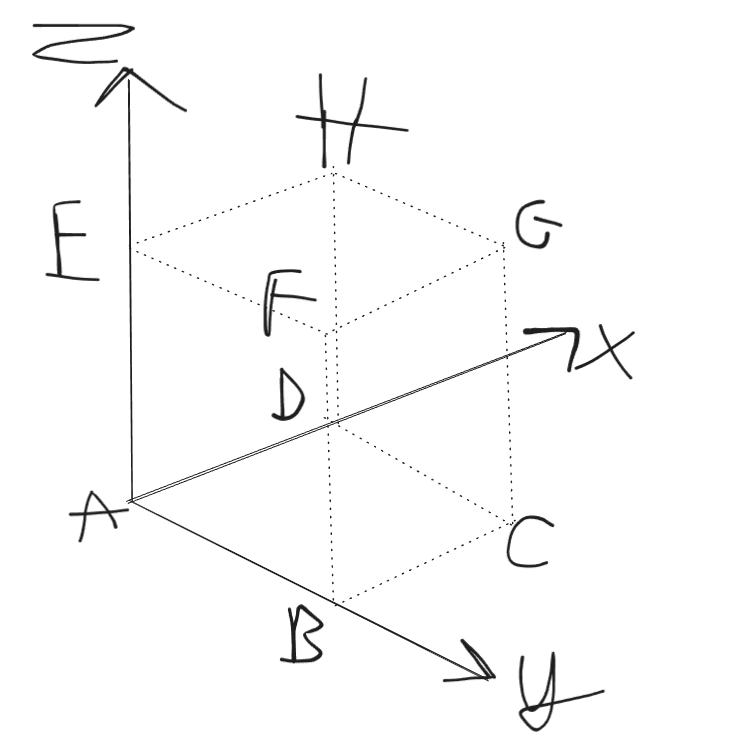
\includegraphics[scale=0.3]{Gregory-1-2-cube.png}
\end{figure}

We would like to calculate the angle between any two diagonals. Let us choose the angle formed
when \(\overrightarrow{AG}\) and \(\overrightarrow{BH}\) intersect. We are working in the standard basis
so we can quickly deduce that:
\begin{equation*}
    \overrightarrow{AG} = [1, 1, 1]
\end{equation*}
\begin{equation*}
    \overrightarrow{BH} = [-1, 1, 1]
\end{equation*}
 
Now we need to calculate the dot product between the two:
\begin{equation*}
    |\overrightarrow{AG}| |\overrightarrow{BH}| \cos(\theta) = \overrightarrow{AG} \cdot \overrightarrow{BH}
\end{equation*}
\begin{equation*}
    \overrightarrow{AG} \cdot \overrightarrow{BH} = -1 + 1 + 1 = 1
\end{equation*}
\begin{equation*}
    |\overrightarrow{AG}| = \sqrt{1 + 1 + 1} = \sqrt{3}
\end{equation*}
\begin{equation*}
    |\overrightarrow{BH}| = \sqrt{1 + 1 + 1} = \sqrt{3}
\end{equation*}

We are interested in \(\theta\) so:
\begin{equation*}
    \cos(\theta) = \frac{1}{\sqrt{3}\sqrt{3}} = \frac{1}{3}
\end{equation*}
\begin{equation*}
    \theta = \cos^{-1}(\frac{1}{3}) \approx 1.23
\end{equation*}

\end{document}
